\chapter{User documentation} \label{ch:docs}

\section{Compiling and running the simulator with Arduino code}

\subsection{Build process and usage examples}

First make sure you comply with the software prerequisites from the section \ref{prerequisits}. Make sure your Boost libraries can be found by the CMake metabuild system from your development environment. For further information, please follow the Boost's getting started guide \cite{boost_get_started}. After that, we can preprocess the sketch, compile it with the simulator, and run the simulator together with the frontend.

\subsubsection{Backend process}
\begin{enumerate}
    \item Run \texttt{preprocess.sh} with the sketch directory. On Windows, use the \texttt{preprocess.bat} script instead. For example:
    
    \begin{lstlisting}[language=shell]
    ./preprocess.sh tests/buttons.
    \end{lstlisting}
    
    \item Build \texttt{backend/CMakeLists.txt}. Available targets are:
    
    \begin{description}
        \item[\texttt{arguino-shared-memory}] for IPC over shared memory
        \item[\texttt{arguino-tcp}] for IPC over TCP connection
        \item[\texttt{arguino}] is an alias for the shared memory version (Default and preferred version).
    \end{description}

    \item Run \footnotemark
    \begin{lstlisting}[language=shell]
    <build dir>/executable/<build target>
    \end{lstlisting}
    
\end{enumerate}

\footnotetext{On Windows, the \texttt{.exe} extension is usually appended, i.e. \texttt{.../<build target>.exe}.}

\subsubsection{Frontend process}
\begin{enumerate}
    \item Build \texttt{frontend/gui.sln}.
    \item Run the \texttt{Gui} executable\footnotemark with the desired scene. For example, in the \texttt{frontend} directory call:
    
    \begin{lstlisting}[language=shell]
    <build dir>/Gui -s ./Scenes/buttons.yaml. 
    \end{lstlisting}
    
    If you built the TCP version of the backend, be sure to add the flag \texttt{-i Tcp}.
    
\end{enumerate}

For frontend and backend to communicate properly, it is necessary that they connect to the same IPC object. For TCP it is the port (\texttt{-p} option for both programs), and for shared memory it is the shared memory's object name (\texttt{-{}-shmem-name} option for both programs). These default to the same value for both of the aforementioned options, port \texttt{8888} and memory named \texttt{Arguino-ipc}.

\footnotetext{\texttt{Gui.exe} on Windows}

\subsection{Command-Line Arguments}
Listed below are all the available command line options for the backend and frontend executables. Default values, if defined, are specified in the square brackets. Expected arguments are in the angle brackets. For arguments accepting only specific enumeration of values, all available values are listed in the angle brackets seperated by a vertical bar (\texttt{|}). In square brackets is the default value used, when the option is omitted.


\subsubsection{Backend}
\begin{description}
    \item[\texttt{-{}-log-simulator <path>}] Path to the log file for simulator events. [\texttt{./core.log}]
    \item[\texttt{-{}-log-ipc <path>}] Path to the log file for Inter-Process Communication (IPC). [\texttt{./core\_ipc.log}]
    \item[\texttt{-v, -{}-verbosity <Debug | Info | Warning | Error>}] Verbosity level of the log files. [\texttt{Info}]
\end{description}

\subsubsection{Frontend}
\begin{description}
    \item[\texttt{-s, -{}-scene <path>}] Path to the \texttt{.yaml} scene definition file. [\texttt{./scene.yaml}]
    \item[\texttt{-c, -{}-components <path>}] Path to the directory containing component definitions. [\texttt{./ComponentManager/Components}]
    \item[\texttt{-i, -{}-ipc <None | Tcp | Shmem>}] Inter-process communication technology utilized for connecting with the simulator. [\texttt{Shmem}]
    \item[\texttt{-{}-log-circuit <path>}] Path to the log file for general circuitry events. [\texttt{./frontend.log}]
    \item[\texttt{-{}-log-ipc <path>}] Path to the log file for IPC events. [\texttt{./frontend\_ipc.log}]
    \item[\texttt{-v, -{}-verbosity <Debug | Info | Warning | Error>}] Verbosity level of the log files. [\texttt{Info}]
\end{description}

\subsubsection{Common for TCP usage}
\begin{description}
    \item[\texttt{-p, -{}-port <int>}] TCP port to listen to. [\texttt{8888}]
\end{description}

\subsubsection{Common for shared memory usage}
\begin{description}
    \item[\texttt{-{}-shmem-name <string>}] Name of the memory-mapped file. [\texttt{Arguino-ipc}]
    \item[\texttt{-{}-shmem-size <int>}] Size of the memory-mapped region per circular buffer, specified in pages (usually $page = 4096B$). [\texttt{1}]
\end{description}

\section{Defining components and scenes} \label{sec:component_spec}
Extensibility of the frontend through custom components and circuits is an important part the project. Here are necessary steps and requirements to create and use new components.

\subsection{Required file structure}
All of the components must reside in one directory, referred to as \textit{definitions directory}. Each component is represented by exactly one directory, referred to as \textit{component directory}, placed in the definitions directory. The definitions directory must be supplied through the \texttt{-c} command line argument. These files must be present in the component directory:

\begin{itemize}
    \item C\# behavior script
    \item YAML component configuration
    \item One or more .svg images
\end{itemize}

The yaml file must have the same name as the component directory, i.e. \texttt{MyComponent/MyComponent.yaml}. The SVGs will be referenced in behavior script by their file name, excluding the .svg extension. For example \texttt{image.svg} will be referred to as \texttt{image}.

\subsubsection{Notes on used YAML notation} \label{yaml_notation}
In the next subsections, we will describe the expected structures of the YAML files using this notation:
\begin{itemize}
  \item angle brackets must be replaced by proper parameters, i.e. \texttt{name: <string>}
  \item properties with question mark are optional, i.e. \texttt{optional?: ...}
  \item Vector2 is represented as a string of 2 float values separated by a space, i.e. \texttt{vector: 7.27 6.9} 
\end{itemize}

\subsection{Component configuration file specification} \label{subsec:component_spec}
This file defines common properties of the custom component type.

\begin{lstlisting}[language=yaml, caption={YAML configuration file structure}]
name: <string>
description?: <string>
imageSize?: <Vector2>
pins?: <uint>
pinNames?:
    - <string>
    - ...
    - ...
\end{lstlisting}

\begin{description}
    \item[\texttt{name}] Name of the component type as displayed in the UI. (not used yet)
    \item[\texttt{description}] Brief description of the component as displayed in the UI. (not used yet)
    \item[\texttt{imageSize}] Desired size of the component's sprites in pixels for default zoom level of the canvas. Defaults to <50, 50>.
    \item[\texttt{pins}] Number of unnamed pins. These pins are identified by their 0-based index in both the scene definition and in the component logic.
    \item[\texttt{pinNames}] List of unique names for each pin. These pins are identified by their given name in both the scene defintion and in the component logic.
\end{description}

\lstinputlisting[language=yaml, caption={Component configuration example: Led.yaml}]{../frontend/ComponentManagement/Components/Led/Led.yaml}

\subsection{Component behavior script specification}
How does the component interact with the rest of the circuit is described by the C\# class with the named the same as the component type. This class must inherit from the abstract \texttt{Component} class. The file containg the class must be added to the \texttt{ComponentManagement.csproj} project. In order to compile, the user's class must also define a constructor like this:

\begin{lstlisting}[language=csharp]
    public #MyComponent#(string definitionPath) 
    : base(definitionPath) { ... }
\end{lstlisting}

However, no code is required in the body of the constructor. The constructor can be used for initialization of properties known before the scene is created. The \texttt{Component} class provides most of the necessary API.

\subsubsection{Component functions and properties}
\begin{description}
    \item[\texttt{virtual void OnInitialized()}]
    Gets called when all of the component instances have been initialized and scene created.

    \item[\texttt{virtual void OnPinConnected(Pin)}]
    Gets called when a component's pin connects to an electric node. The connected pin is passed as argument.

    \item[\texttt{virtual void OnPinDisconnected(Pin)}]
    Gets called when a component's pin disonnects from an electric node. The disconnected pin is passed as argument.

    \item[\texttt{virtual void OnPinStateChanged(Pin)}]
    Gets called when a component's pin detected a change in digital state of a node it has been connected to. It can be thought of as changing input value on the pin. Pins set to WriteOnly mode by design don't detect this change. The detected pin is passed as argument.

    \item[\texttt{virtual void OnControlPress(Vector2)}]
    Gets called when the component has been pressed on the circuit canvas. The cursor position at the time of the press is passed as argument.

    \item[\texttt{virtual void OnControlRelease}]
    Gets called when the component has been released on the circuit canvas.

    \item[\texttt{void UpdateSprite(string)}]
    Changes the .svg image drawn to the canvas. The new image is given by the svg name specified in the argument.

    \item[\texttt{Pin? GetPin(string)}]
    Returns a Pin object with the name given in the argument. The name must be defined in the component's \texttt{namedPins} list. Returns null if no such pin exists.

    \item[\texttt{Pin? GetPin(uint)}]
    Returns a Pin object with the id given in the argument. The allowed range of Ids is from \texttt{0} to $pins + namedPins.Length$. With unnamed pins starting from the id \texttt{0} and named pins starting from the id \texttt{pins}. Returns null if the pin id is out of range.
\end{description}

\subsubsection{Pin functions and properties}
\begin{description}
    \item[\texttt{uint Pin.Id}]
    Id of the pin, as described in the \texttt{GetPin(uint)} section.

    \item[\texttt{string Pin.Name}]
    Name of the pin as described in the component configuration.

    \item[\texttt{bool Pin.IsDriving}]
    True if the pin is driving. That is, if it actively forces the digital state on the connected node to be high. If the node has at least 1 driving pin, it's digital state will be high. It will be low otherwise.

    \item[\texttt{bool Pin.IsHigh}]
    True if the digital state of the connected node is high.

    \item[\texttt{bool Pin.IsLow}]
    True if the digital state of the connected node is low.

    \item[\texttt{bool Pin.IsWriteOnly}]
    Write only pins don't react to changes in the connected node's digital state.

    \item[\texttt{bool Pin.IsReadOnly}]
    Read only pins cannot be set to driving.

    \item[\texttt{bool Pin.IsConnected}]
    Whether is the pin connected to any electrical node.

    \item[\texttt{void Pin.MakeReadOnly()}]
    Sets the pin to read only mode. Read only pins cannot be set to driving.

    \item[\texttt{void Pin.MakeWriteOnly()}]
    Sets the pin to write only mode. Write only pins don't react to changes in the connected node's digital state.

    \item[\texttt{void Pin.MakeGeneral()}]
    Sets the pin to general mode. General pins don't pose any restrictions to reading or writing.

    \item[\texttt{void Pin.SetValue(bool)}]
    If the argument is true, it sets the pin to be driving. Otherwise, the pin set to not drive.

    \item[\texttt{void Pin.SetHigh()}]
    Sets the pin to be driving. Same as \texttt{SetValue(true)}.

    \item[\texttt{void Pin.SetLow()}]
    Sets the pin to be not driving. Same as \texttt{SetValue(false)}.
\end{description}

\subsection{Defining scenes} \label{subsec:scene_spec}
The scene YAML file describes component instances present in the scene, and how are their pins connected together in nodes. The path of this file is supplied through the \texttt{-s} command line argument. There are no restriction to where the scene file has to be placed.

\begin{lstlisting}[language=yaml, caption={YAML scene file structure}]
components:
  <Type name>:
    <Instance name>:
      position: <Vector2>
      rotation?: <float>
      scale?: <Vector2>
    <Instance name>:
      ...
nodes:
  - [ <Instance name>.<Pin name>, ...]
  - ...
  - ...
\end{lstlisting}

\begin{description}
    \item[\texttt{components}]
    Dictionary of component type objects. These objects are dictionaries of component instances of that type. These instances define properties of the individual components. 

    \item[\texttt{Type name}]
    String. Name of the component type. This must match the component directory name.

    \item[\texttt{Instance name}]
    String. Name of the component instance. It identifies the instance within the node definition and in the UI. It must be unique across all instances within the components dictionary.

    \item[\texttt{position}]
    Coordinates on the circuit canvas, with origin in the upper left corner.

    \item[\texttt{rotation}]
    Clockwise rotation angle in degrees on the circuit canvas.

    \item[\texttt{scale}]
    Relative scaling along x an y axis on the circuit canvas.

    \item[\texttt{nodes}]
    List of lists. The inner list represents all pins connected to the same electrical node. Its element is an instance-pin pair separated by a dot. Instance name must be present in the components dictionary. Pin name must be present in the component's configuration. In the case of unnamed pins, pin name is simply its index.
\end{description}

\lstinputlisting[language=yaml, caption={Scene example: minimal.yaml}, label={lst:scene}]{../frontend/Scenes/minimal.yaml}

The example scene in the listing \ref{lst:scene} contains 2 LEDs, 1 button and 1 source of voltage. Source, which has one pin that is always driving, is connected to the 0th pin of the button, which reads a high value of the node. Both LEDs are connected to the 1st pin of the same button. Pressing the button will copy the digital state from pin 0 to pin 1, pin 1 becomes driving, and thus lights up the LEDs.

\section{IPC interface}
This section describes how to set up IPC communication of a custom frontend application with the backend simulator. The two processes can communicate together either via TCP connection or through shared memory. The only requirement for a TCP connection, is that the client on the frontend listens to the same port as the server on the backend. IPC over shared memory requires a few more considerations, so that the memory accesses match the memory layout of shared internal structure created by the backend. This structure is described in the subsection \ref{shmem_specs};

The processes communicate using concrete events with up to 3 integer arguments. These events are encoded into a human readable text messages, seperated by a common delimeter. The messages are then sent over IPC.

\subsection{Text message format}
Individual messages are delimited by the semicolon character (\texttt{;}). The individual values within one message are delimited by the colon character (\texttt{:}). The integer values are written in decimal system, using the ASCII characters of the actual digits. The semantics of these values are better described in the chapter about architecture, subsection \ref{subsec:events}. The format of the message then looks as the following:

\begin{lstlisting}[
    caption={Format of an IPC text message},
    literate={:}{{\color{Bittersweet}{:}\color{Black}}}1
             {;}{{\color{Brown}{;}\color{Black}}}1
]
    <sim_time>:<lvt>:<event_type>:<arg1>:<arg2>:<arg3>;
\end{lstlisting}

\begin{description}
    \item[\texttt{sim\_time}] Simulation time, 64-bit signed integer. Real time elapsed from the start of the backend's simulation represented in microseconds. The backend has no use for this value.
    \item[\texttt{lvt}] Local virtual time, 64-bit signed integer. It describes an order in which the event occured, relative to other events.
    \item[\texttt{event\_type}] A single character representing the type of the event. This type decides the action taken upon consuming the event. Recognized event types and their corresponding characters are described in the next subsection.
    \item[\texttt{arg1, arg2, arg3}] 32-bit signed integers. Values have meaning depending on the event. Arguments not defined by the event type can be omitted. Make sure that the number of colons match the number of passed arguments.
\end{description}

For example, this next message encodes the \texttt{Write} event passing 2 arguments at the simulation time of 264 seconds:

\begin{lstlisting}[
    caption={Example of an IPC text message},
    literate={:}{{\color{Bittersweet}{:}\color{Black}}}1
             {;}{{\color{Brown}{;}\color{Black}}}1
]
    000264997488:0000016:W:08:1;
\end{lstlisting}

\xxx{Decide on whether to describe or remove the zero paddings}.

\subsection{Recognized event types}

\subsubsection{Write event}
Signalizes digital value being written into a pin. If consumed by the backend, the value gets written to the internal \texttt{ArduinoState}. If consumed by the frontend, it should reflect the changes caused by the change of the pin's state. This event is produced by the backend on \texttt{digitalWrite} function call within the sketch.

\begin{description}
    \item[Encoding character:] \texttt{W}
    \item[Arguments:] \hfill
    \begin{description}
        \item[1: Pin index] of the digital pin from the range 0--13.
        \item[2: Value] 0 for the low value, 1 for the high value.
    \end{description}
\end{description}

\subsubsection{Pinmode event}
Signalizes change of a pin mode of a pin. If consumed by the backend the value gets written to the internal \texttt{Arduinostate}. If consumed by the frontend, it should change the behavior of the pin, such that only input pins are able to send the \texttt{Write} event. This event is produced by the backend on \texttt{pinMode} function call within the sketch.

\begin{description}
    \item[Encoding character:] \texttt{P}
    \item[Arguments:] \hfill
    \begin{description}
        \item[1: Pin index] of the digital pin from the range 0--13.
        \item[2: Mode] 0 for the output mode, 1 for the input mode.
    \end{description}
\end{description}

\subsubsection{Reboot event}
Produced by the backend, when the simulation has started over. Useful, when the backend process has be
terminated and then executed again. At this point the frontend has to invalidate its current state and start again. Backend itself does no action upon consuming this event (it may force the reboot of the simulation in the future).

\begin{description}
    \item[Encoding character:] \texttt{R}
    \item[Arguments:] None
\end{description}

\subsection{Shared memory specification} \label{shmem_specs}

\subsubsection{Locating memory mapped file}
On Linux, the mapped memory region is orchestrated by a proper shared memory object. It can be accessed either by a syscall, or by reading the \texttt{\textbackslash{}dev\textbackslash{}shm\textbackslash{}<shmem\_name>} virtual file.

On Windows, the shared memory is emulated by the \texttt{Boost.interprocess} library via a memory mapped file. It can be located at the path specified by the \texttt{Common AppData} registry. For Windows Vista and newer, this path defaults to \texttt{C:\textbackslash{}ProgramData}. On this path, a \texttt{boost\_interprocess} directory is created. The memory mapped file, named the same as the shared memory object, can be found in one if its subdirectories. \cite{boost_shared_memory}

In either case, the name of the read memory mapped file or shared memory object has to match the name given to the mapped region via the \texttt{-{-}shmem-name} flag of the backend command.

\subsubsection{Memory layout}

\begin{figure}
    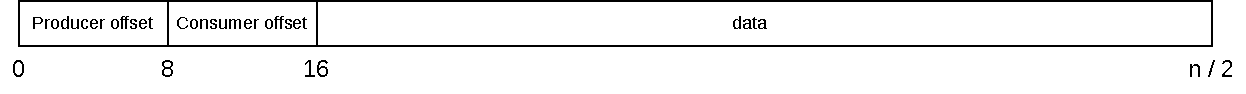
\includegraphics[width=\textwidth, keepaspectratio]{img/circular-buffer-memory.pdf}
    \caption{Memory layout of the circular buffer}
    \label{fig:circular-buffer-memory}
\end{figure}

The mapped memory region is split into 2 equal sections, both containg the same circular buffer data structure. So for a mapped region of size $n$ bytes, and for the start address of the region $s_a$, the second buffer is located on the memory address $s_a + n/2$ ($n$ is always even, as it is a multiple of a page size). Let's denote the start address of a buffer $s_b$

The buffer itself has 2 control variables stored within it. Both are 64-bit unisgned integers representing an offset within the buffers data. The first, located at $s_b$, is the offset at which the producer will write the next chunk of data into the buffer. The second, located at $s_b + 8$, is the offset at which the next chunk of data will be read from the buffer, if present. From the address $s_b + 16$ until the next buffer, or the end of the mapped region, the actual data are stored. That means the actual capacity of data stored within one buffer is $n/2 - 16$.

The data have no uniform size, structure or address alignment. The length of a message in the buffer must be deduced from the data within the message itself. In case of the text encoding, it is the message delimeter. A message can be located at the boundary of the data region. In that case the message is split so that every byte until the very end of the region is filled, and the rest is written at $s_b + 16$ again. There are no gaps between the messages.

The frontend process is responsible for consuming messages from the first buffer and producing them to the second one. As such, the consumer offset of the first buffer and the producer offset of the second buffer must be updated accordingly. The other two offsets must remain read only. The backend process has these roles reversed.

